% Options for packages loaded elsewhere
\PassOptionsToPackage{unicode}{hyperref}
\PassOptionsToPackage{hyphens}{url}
%
\documentclass[
]{article}
\usepackage{lmodern}
\usepackage{amssymb,amsmath}
\usepackage{ifxetex,ifluatex}
\ifnum 0\ifxetex 1\fi\ifluatex 1\fi=0 % if pdftex
  \usepackage[T1]{fontenc}
  \usepackage[utf8]{inputenc}
  \usepackage{textcomp} % provide euro and other symbols
\else % if luatex or xetex
  \usepackage{unicode-math}
  \defaultfontfeatures{Scale=MatchLowercase}
  \defaultfontfeatures[\rmfamily]{Ligatures=TeX,Scale=1}
\fi
% Use upquote if available, for straight quotes in verbatim environments
\IfFileExists{upquote.sty}{\usepackage{upquote}}{}
\IfFileExists{microtype.sty}{% use microtype if available
  \usepackage[]{microtype}
  \UseMicrotypeSet[protrusion]{basicmath} % disable protrusion for tt fonts
}{}
\makeatletter
\@ifundefined{KOMAClassName}{% if non-KOMA class
  \IfFileExists{parskip.sty}{%
    \usepackage{parskip}
  }{% else
    \setlength{\parindent}{0pt}
    \setlength{\parskip}{6pt plus 2pt minus 1pt}}
}{% if KOMA class
  \KOMAoptions{parskip=half}}
\makeatother
\usepackage{xcolor}
\IfFileExists{xurl.sty}{\usepackage{xurl}}{} % add URL line breaks if available
\IfFileExists{bookmark.sty}{\usepackage{bookmark}}{\usepackage{hyperref}}
\hypersetup{
  pdfauthor={Erick Robinson1,; Kyle Bocinsky2,3; Darcy Bird4; Jacob Freeman1; Robert L. Kelly5},
  pdfkeywords={true},
  hidelinks,
  pdfcreator={LaTeX via pandoc}}
\urlstyle{same} % disable monospaced font for URLs
\usepackage[margin=1in]{geometry}
\usepackage{longtable,booktabs}
% Correct order of tables after \paragraph or \subparagraph
\usepackage{etoolbox}
\makeatletter
\patchcmd\longtable{\par}{\if@noskipsec\mbox{}\fi\par}{}{}
\makeatother
% Allow footnotes in longtable head/foot
\IfFileExists{footnotehyper.sty}{\usepackage{footnotehyper}}{\usepackage{footnote}}
\makesavenoteenv{longtable}
\usepackage{graphicx}
\makeatletter
\def\maxwidth{\ifdim\Gin@nat@width>\linewidth\linewidth\else\Gin@nat@width\fi}
\def\maxheight{\ifdim\Gin@nat@height>\textheight\textheight\else\Gin@nat@height\fi}
\makeatother
% Scale images if necessary, so that they will not overflow the page
% margins by default, and it is still possible to overwrite the defaults
% using explicit options in \includegraphics[width, height, ...]{}
\setkeys{Gin}{width=\maxwidth,height=\maxheight,keepaspectratio}
% Set default figure placement to htbp
\makeatletter
\def\fps@figure{htbp}
\makeatother
\setlength{\emergencystretch}{3em} % prevent overfull lines
\providecommand{\tightlist}{%
  \setlength{\itemsep}{0pt}\setlength{\parskip}{0pt}}
\setcounter{secnumdepth}{5}
\usepackage[labelfont={bf}]{caption}
\newlength{\cslhangindent}
\setlength{\cslhangindent}{1.5em}
\newenvironment{cslreferences}%
  {\setlength{\parindent}{0pt}%
  \everypar{\setlength{\hangindent}{\cslhangindent}}\ignorespaces}%
  {\par}

\title{true}
\author{Erick Robinson\textsuperscript{1,*} \and Kyle Bocinsky\textsuperscript{2,3} \and Darcy Bird\textsuperscript{4} \and Jacob Freeman\textsuperscript{1} \and Robert L. Kelly\textsuperscript{5}}
\date{April 17, 2020}

\begin{document}
\maketitle
\begin{abstract}
The northern American Southwest provides one of the most well-documented cases of human population growth and decline in the world. The geographic extent of this decline in North America is unknown due to the lack of high-resolution palaeodemographic data from regions across and beyond the greater Southwest, where archaeological radiocarbon data is often the only available proxy for investigating these palaeodemographic processes. Radiocarbon time series across and beyond the greater Southwest suggest widespread population collapses from AD 1300--1600. However, radiocarbon data have potential biases caused by variable radiocarbon sample preservation, sample collection, and the non-linearity of the radiocarbon calibration curve. In order to be confident in the wider trends seen in radiocarbon time series across and beyond the greater Southwest, here we focus on regions that have multiple palaeodemographic proxies and compare those proxies to radiocarbon time series. We develop a new method for time series analysis and comparison between dendrochronological data and radiocarbon data. Results confirm a multiple proxy decline in human populations across the Upland US Southwest, Central Mesa Verde, and Northern Rio Grande from AD 1300--1600. These results lend confidence to single proxy radiocarbon-based reconstructions of paleodemography outside the Southwest that suggest post-AD 1300 population declines in many parts of North America.
\end{abstract}

\textsuperscript{1} Utah State University\\
\textsuperscript{2} Crow Canyon Archaeological Center\\
\textsuperscript{3} University of Montana\\
\textsuperscript{4} Washington State University\\
\textsuperscript{5} University of Wyoming

\textsuperscript{*} Correspondence: \href{mailto:erick.robinson@usu.edu}{Erick Robinson \textless{}\href{mailto:erick.robinson@usu.edu}{\nolinkurl{erick.robinson@usu.edu}}\textgreater{}}

\newpage

\hypertarget{introduction}{%
\section*{Introduction}\label{introduction}}
\addcontentsline{toc}{section}{Introduction}

The spatial and temporal ubiquity of archaeological radiocarbon dates makes them an unprecedented proxy for human paleodemography. The past decade has witnessed a rapid increase in the use of archaeological radiocarbon time series to reconstruct prehistoric population growth and decline in various regions of the world (Bevan et al., \protect\hyperlink{ref-Bevan2019}{2019}; Crema et al., \protect\hyperlink{ref-Crema2016}{2016}; Goldberg et al., \protect\hyperlink{ref-Goldberg2016}{2016}; Palmisano et al., \protect\hyperlink{ref-Palmisano2019}{2019}; Peros et al., \protect\hyperlink{ref-Peros2010}{2010}; Russell and Steele, \protect\hyperlink{ref-Russell2009}{2009}; Shennan et al., \protect\hyperlink{ref-Shennan2013}{2013}; Wang et al., \protect\hyperlink{ref-Wang2014}{2014}; Williams, \protect\hyperlink{ref-Williams2012}{2012}). One of the first aggregations of radiocarbon dates for palaeodemographic analysis was by Berry (Berry, \protect\hyperlink{ref-Berry1982}{1982}) in his study of population growth, decline and migration across the American Southwest. Radiocarbon time series were used as a complement to earlier periods that lacked robust dendrochronological records. Berry (\protect\hyperlink{ref-Berry1982}{1982}: 120) noted that they were ``not even remotely related to population size'', but rather the ``relative probability of occupation through time'' and ``the major trends in these charts (i.e., peaks and troughs) should provide a reliable indication of the direction of change''. Later, Rick (\protect\hyperlink{ref-Rick1987}{1987}: 56) more formally outlined the use of radiocarbon time series as a method for paleodemography by developing an `inference chain' that detailed the various biases involved in their use and interpretation. Rick identified three biases: creation bias, preservation bias, and investigation bias (Rick, \protect\hyperlink{ref-Rick1987}{1987}). Over the past decade, as archaeologists have assembled and analysed large radiocarbon datasets from various regions of the world, there has been considerable focus on these biases, notably creation (Crombé and Robinson, \protect\hyperlink{ref-Crombe2014}{2014}; Freeman, Byers, et al., \protect\hyperlink{ref-Freeman2018}{2018}; Naudinot et al., \protect\hyperlink{ref-Naudinot2014}{2014}) and preservation bias (Bluhm and Surovell, \protect\hyperlink{ref-Bluhm2019}{2019}; Peros et al., \protect\hyperlink{ref-Peros2010}{2010}; Surovell and Brantingham, \protect\hyperlink{ref-Surovell2007}{2007}; Surovell et al., \protect\hyperlink{ref-Surovell2009}{2009}; Williams, \protect\hyperlink{ref-Williams2012}{2012}), as well as bias caused by the radiocarbon calibration process (Armit et al., \protect\hyperlink{ref-Armit2013}{2013}; Bamforth and Grund, \protect\hyperlink{ref-Bamforth2012}{2012}; Contreras and Meadows, \protect\hyperlink{ref-Contreras2014}{2014}; Michczynski and Michczynska, \protect\hyperlink{ref-Michczynski2006}{2006}; Timpson et al., \protect\hyperlink{ref-Timpson2014}{2014}; Williams, \protect\hyperlink{ref-Williams2012}{2012}). Of the three biases Rick identified, investigation bias has been the most understudied thus far. Investigation bias occurs when investigators gather more radiocarbon samples for particular periods of time or specific geographic regions, which leads to periods or regions with more or less radiocarbon representation than the average time period or region. The biased selection of radiocarbon samples would then appear to be relative increases or decreases in population when they are merely artefacts of research history and fieldwork practice. Investigation bias has been understudied because for many regions of the world radiocarbon data are the only currently available proxy evidence enabling reconstructions of paleodemography in continuous time series spanning millennia. Assessing the impact of investigation bias on radiocarbon-based reconstructions of paleodemography requires comparison with other paleodemographic proxies.

The American Southwest provides one the best available case studies for assessing the role of investigation bias in radiocarbon-based reconstructions of paleodemography. It also has one of the most well-documented cases of population growth and decline in the world (Bocinsky et al., \protect\hyperlink{ref-Bocinsky2016}{2016}; Freeman, Baggio, et al., \protect\hyperlink{ref-Freeman2018PNAS}{2018}; Hill et al., \protect\hyperlink{ref-Hill2004}{2004}; Kohler et al., \protect\hyperlink{ref-Kohler2010b}{2010}; Robinson et al., \protect\hyperlink{ref-Robinson2019}{2019}). For almost a century, researchers have collected multiple proxies, such as dendrochronological records, settlement size records, and ceramic seriation records to address the magnitude of this population growth and decline. However, a critical knowledge gap still exists for the exact scale of population decline across and beyond the Southwest (Boyer et al., \protect\hyperlink{ref-Boyer2010}{2010}; Cameron, \protect\hyperlink{ref-Cameron2010}{2010}). This gap is because the less intensively researched regions lack multiple proxies for robust reconstructions of paleodemography. In these regions, radiocarbon data are the only available proxy time series for reconstructing paleodemography. Over the past six years, we have collected all available radiocarbon data across and beyond the Southwest (Robinson et al., \protect\hyperlink{ref-Robinson2019}{2019}). Initial analyses of this new radiocarbon dataset have revealed extensive population decline from AD 1300--1600 across and beyond the Southwest (Freeman, Baggio, et al., \protect\hyperlink{ref-Freeman2018PNAS}{2018}; Robinson et al., \protect\hyperlink{ref-Robinson2019}{2019}). Therefore, the geographic extent of Late Prehistoric population decline could be much broader than previously expected.

The potential importance of this widespread population decline for research on Late Prehistoric archaeology of the American West requires comparison of the sensitivity of lower-resolution radiocarbon data against other higher-resolution palaeodemographic proxies. In the most well-documented regions (such as the northern American Southwest) we expect radiocarbon records to reflect the highest amount of investigation bias, as researchers have the option of selecting from a suite of other higher-resolution proxies, including dendrochronology and ceramic seriation. Investigation bias can create an artificial `edge effect' spuriously appearing as a decrease in population. Here we develop a new method for arraying dendrochronological records as time series for comparison against radiocarbon time series. We focus on the broader region of the Upland US Southwest (UUSW) for which there is a robust dendrochronological record (Bocinsky et al., \protect\hyperlink{ref-Bocinsky2016}{2016}).

We also focus on the more concentrated and intensively investigated Central Mesa Verde (CMV) and Northern Rio Grande (NRG) regions of the UUSW (Figure \ref{fig:Figure1}), for which multiproxy palaeodemographic reconstructions were produced by the Village Ecodynamics Project (VEP) (Ortman, \protect\hyperlink{ref-Ortman2016}{2016}; Schwindt et al., \protect\hyperlink{ref-Schwindt2016}{2016}). The VEP is an interdisciplinary, multi-method research initiative aimed at better understanding demography of ancestral Pueblo farmers and human-environment interaction across the UUSW. As part of the project, VEP researchers cataloged data on all known archaeological habitation sites within a 4,600-km2 area in the CMV (Schwindt et al., \protect\hyperlink{ref-Schwindt2016}{2016}) and a 6,900-km2 area in the NRG (Ortman, \protect\hyperlink{ref-Ortman2016}{2016}), to which most of the CMV population migrated during the thirteenth century AD (Ortman, \protect\hyperlink{ref-Ortman2016}{2016}). They integrated data including pitstructure and room count estimates, the presence of diagnostic architectural features, surface ceramic tallies, surveyor assessments, and limited dendrochronological data in an empirical Bayesian framework to develop population estimates for each region resolved to periods ranging from 20 to 125 years in length (Ortman, \protect\hyperlink{ref-Ortman2016}{2016}; Schwindt et al., \protect\hyperlink{ref-Schwindt2016}{2016}). The VEP estimates are the highest quality regional palaeodemographic reconstructions currently available in the UUSW, and are completely independent of the radiocarbon records for the region. They are therefore useful in exploring the impact of investigation bias in the radiocarbon record.



\begin{figure}

{\centering 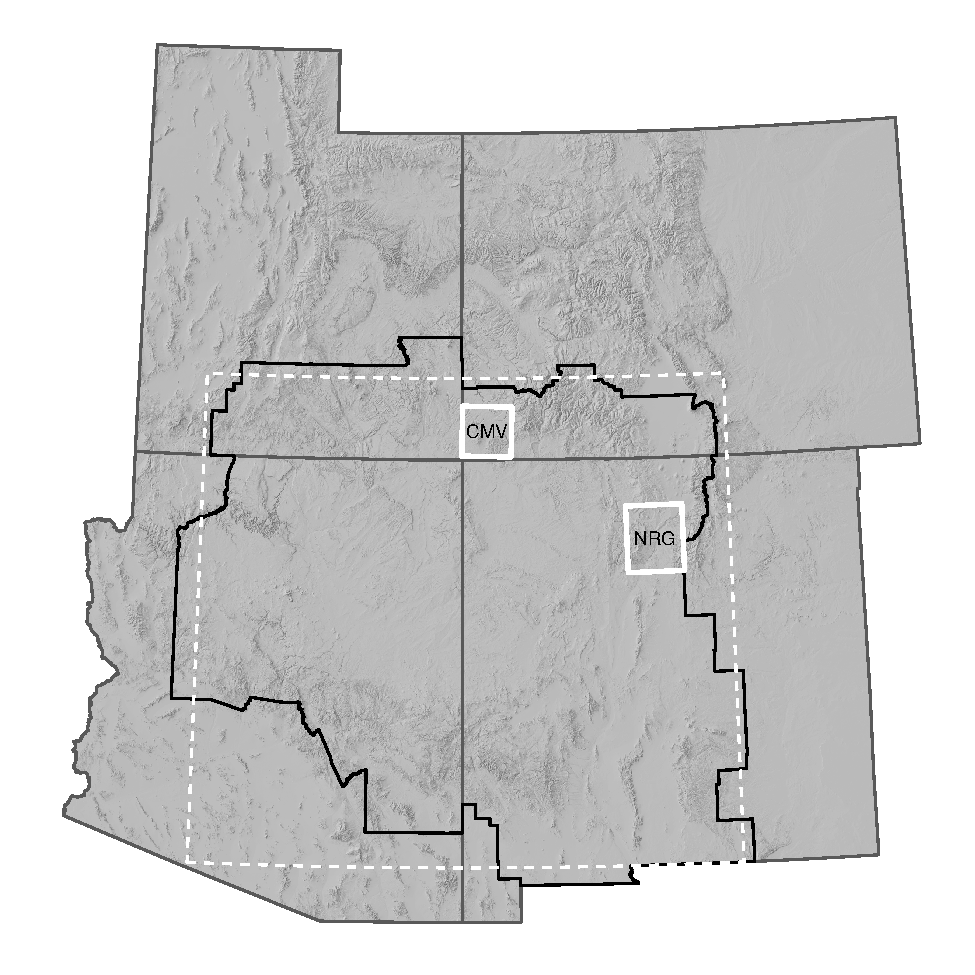
\includegraphics[width=0.5\linewidth]{/Users/bocinsky/git/publications/robinson2020/analysis/figures/Figure1-1} 

}

\caption{The UUSW as defined in this study (region with black border). The white dashed area represents the UUSW as defined by Bocinsky et al. (\protect\hyperlink{ref-Bocinsky2016}{2016}). VEP study areas are white boxes. CMV: Central Mesa Verde; NRG: Northern Rio Grande.}\label{fig:Figure1}
\end{figure}

We expect that substantial investigation bias is present in radiocarbon records if those records substantially diverge from the dendrochronological and multiproxy reconstructions. If the lower-resolution radiocarbon records reveal similar trends to the two other records, we expect investigation bias does not substantially impact the ability of radiocarbon records to be used as relative measures of the directionality of population change through time. This would, in turn, lend more confidence to radiocarbon records across the American West that reveal extensive post AD 1300 population declines but lack other palaeodemographic proxies.

\hypertarget{methods}{%
\section*{Methods}\label{methods}}
\addcontentsline{toc}{section}{Methods}

Here we compare two large collections of radiocarbon and tree-ring dates drawn from the UUSW. After harmonizing those datasets with one another and calibrating the radiocarbon dates, we calculate binned summed probability distributions across the UUSW, CMV, and NRG. The radiocarbon dates we analyse here are drawn from the National Science Foundation supported project, ``Populating a Radiocarbon Database for North America,'' which have been uploaded to the Canadian Archaeological Radiocarbon Database (CARD; \url{https://www.canadianarchaeology.ca}). Tree-ring data are those presented by Bocinsky et al. (\protect\hyperlink{ref-Bocinsky2016}{2016}). Both datasets are available on the Digital Archaeological Record (see \protect\hyperlink{data-accessibility}{Data Accessibility}).

\hypertarget{study-area}{%
\subsection*{Study Area}\label{study-area}}
\addcontentsline{toc}{subsection}{Study Area}

The UUSW was geographically defined by Bocinsky et al. (\protect\hyperlink{ref-Bocinsky2016}{2016}) as the region between 105--113°W and 32--38°N. Here, we refine that definition in two ways. First, because location data for our radiocarbon database are only resolved to the county level for most sites (Robinson et al., \protect\hyperlink{ref-Robinson2019}{2019}), we define our study region to include all counties whose geographic centroids fall within the region from Bocinsky et al. (\protect\hyperlink{ref-Bocinsky2016}{2016}). Second, because of the generally poor tree-ring date record in the Sonoran Desert, we exclude the Phoenix and Tucson basins by dropping Maricopa, Pinal, and Pima counties in Arizona. Figure \ref{fig:Figure1} shows the original UUSW from Bocinsky et al. (\protect\hyperlink{ref-Bocinsky2016}{2016}) and revised study area used in this analysis, as well as the two VEP study areas.

\hypertarget{period-of-interest}{%
\subsection*{Period of Interest}\label{period-of-interest}}
\addcontentsline{toc}{subsection}{Period of Interest}

Here, we focus our analyses on the period for which data are most abundant: 1750--150 BP, or AD 200--1800. This period includes the periods of the VEP population estimates for the CMV (AD 600--1280) and NRG (AD 900--1760), and extends 400 years earlier than the CMV estimates to allow us to assess trends in the radiocarbon record leading up to the VEP reconstructions, and to control for edge effects. While the VEP demographic estimates are for ancestral Pueblo populations only, it is likely that the tree-ring records include samples from Spanish colonial contexts after AD 1600 or so.

\hypertarget{datasets}{%
\subsection*{Datasets}\label{datasets}}
\addcontentsline{toc}{subsection}{Datasets}

We cleaned the radiocarbon database by first removing all non-archaeological dates. To ensure our data are reasonably precise, we removed all radiocarbon dates with 1σ errors greater than 300 years and more than 25\% of the uncalibrated age. We removed dates with duplicate lab numbers whose radiocarbon ages, 1σ errors, or county information did not match. We then trimmed these data to counties within the UUSW. We retained radiocarbon dates that likely derive from our period of interest by first calibrating all of the dates, then retaining dates whose 95\% calibrated probability masses overlapped 1750--150 BP.

We draw on the tree-ring date database presented by Bocinsky et al. (\protect\hyperlink{ref-Bocinsky2016}{2016}). These data were compiled by Tim Kohler and Rebecca Higgins from many contributors, and the vast majority of dates were produced by the Laboratory of Tree Ring Research at the University of Arizona. The original dataset contained 32,863 cutting, near-cutting, and non-cutting dates from across the US Southwest. Here, we only use the dates that are most likely to be accurate --- cutting dates (`B', `G', `L', `c', or `r' dates, with or without a `+') for which we know the year the tree died, and near-cutting dates (`v' or `v+' dates) which are likely within 0--3 years of the true date of the outermost ring. The Bocinsky et al. (\protect\hyperlink{ref-Bocinsky2016}{2016}) data contain site locations; for this analysis, we first spatially cropped the database to our study area, and then translated those locations to the county level. We converted the original date determinations to BP to match calibrated radiocarbon year conventions, and retained dates within 1750--150 BP.

Finally, due to much of the radiocarbon data only being resolved to the county level, we had to approximate inclusion in the VEP, CMV and NRG study areas. The CMV study area conforms well to Montezuma county, Colorado; the NRG overlaps with Los Alamos, Rio Arriba, Sandoval, Santa Fe, and Taos counties in New Mexico. In the analyses below, dates were included as ``within'' each study area if they derive from those respective counties.

Our final dataset includes 1,531 radiocarbon dates from 482 unique sites, dating from 2260--90 BP (uncalibrated; 309 BC--1860 AD) and 15,077 tree-ring dates from 770 unique sites, dating from 1749--152 BP (201--1798 AD). Table \ref{tab:Table1} presents the counts of dates and sites of each date type in the CMV and NRG study areas.

\begin{table}

\caption{\label{tab:Table1}Counts of radiocarbon and tree-ring dates and sites in this study.}
\centering
\begin{tabular}[t]{lrrrr}
\toprule
\multicolumn{1}{c}{ } & \multicolumn{2}{c}{Radiocarbon} & \multicolumn{2}{c}{Tree-ring} \\
\cmidrule(l{3pt}r{3pt}){2-3} \cmidrule(l{3pt}r{3pt}){4-5}
Study Area & Dates & Sites & Dates & Sites\\
\midrule
UUSW Total & 1,531 & 482 & 15,077 & 770\\
CMV & 36 & 18 & 4,435 & 219\\
NRG & 83 & 40 & 2,306 & 146\\
\bottomrule
\end{tabular}
\end{table}

Date densities across the study area were very uneven, with high counts of radiocarbon dates deriving from Navajo County, Arizona, and almost a third of the tree-ring dates in our study being from Montezuma County, Colorado. Below, we overcome some of these sampling issues by binning dates by site and occupation phase. Still, these disparities likely demonstrate more fundamental differences in research design across archaeological projects. There are very few radiocarbon dates from the two VEP study areas, indicating a clear bias towards using tree-ring dating where (and when) possible. Figure \ref{fig:Figure2} presents the number of radiocarbon and tree-ring dates by county within our study area. Figure \ref{fig:Figure3} presents the number of unique sites with radiocarbon and tree-ring dates by county within our study area. There are similar ratios of radiocarbon dates to sites with radiocarbon dates for the CMV and NRG (roughly 2:1), but sites in the CMV tend to have a third more tree-ring dates than those in the NRG (20:1 versus 15:1, respectively).

\begin{figure}

{\centering 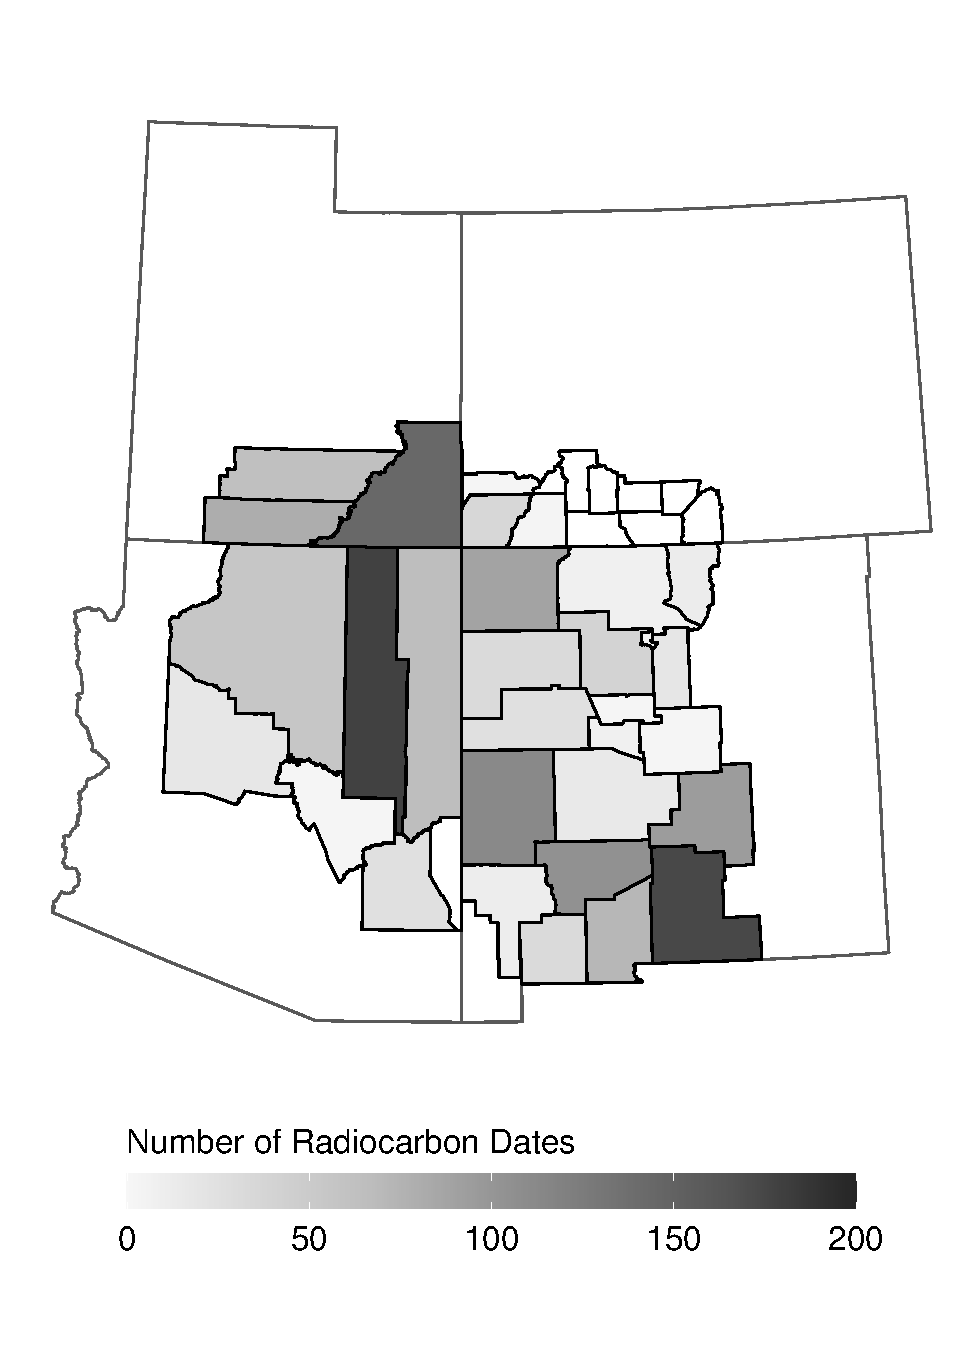
\includegraphics[width=0.45\linewidth]{/Users/bocinsky/git/publications/robinson2020/analysis/figures/Figure2-1} 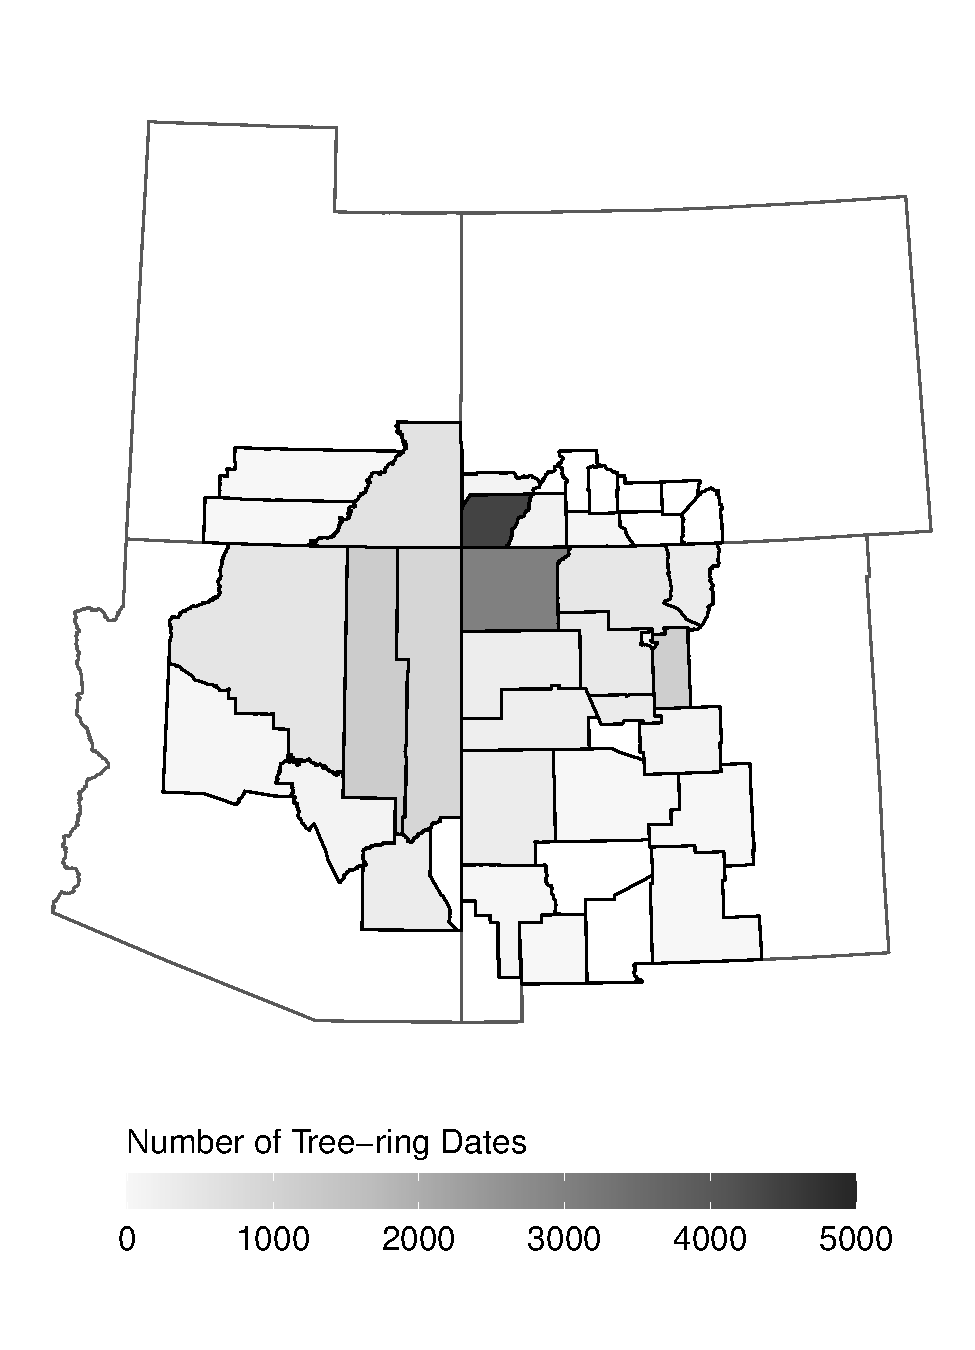
\includegraphics[width=0.45\linewidth]{/Users/bocinsky/git/publications/robinson2020/analysis/figures/Figure2-2} 

}

\caption{The number of radiocarbon and tree-ring dates by county in this study.}\label{fig:Figure2}
\end{figure}

\begin{figure}

{\centering 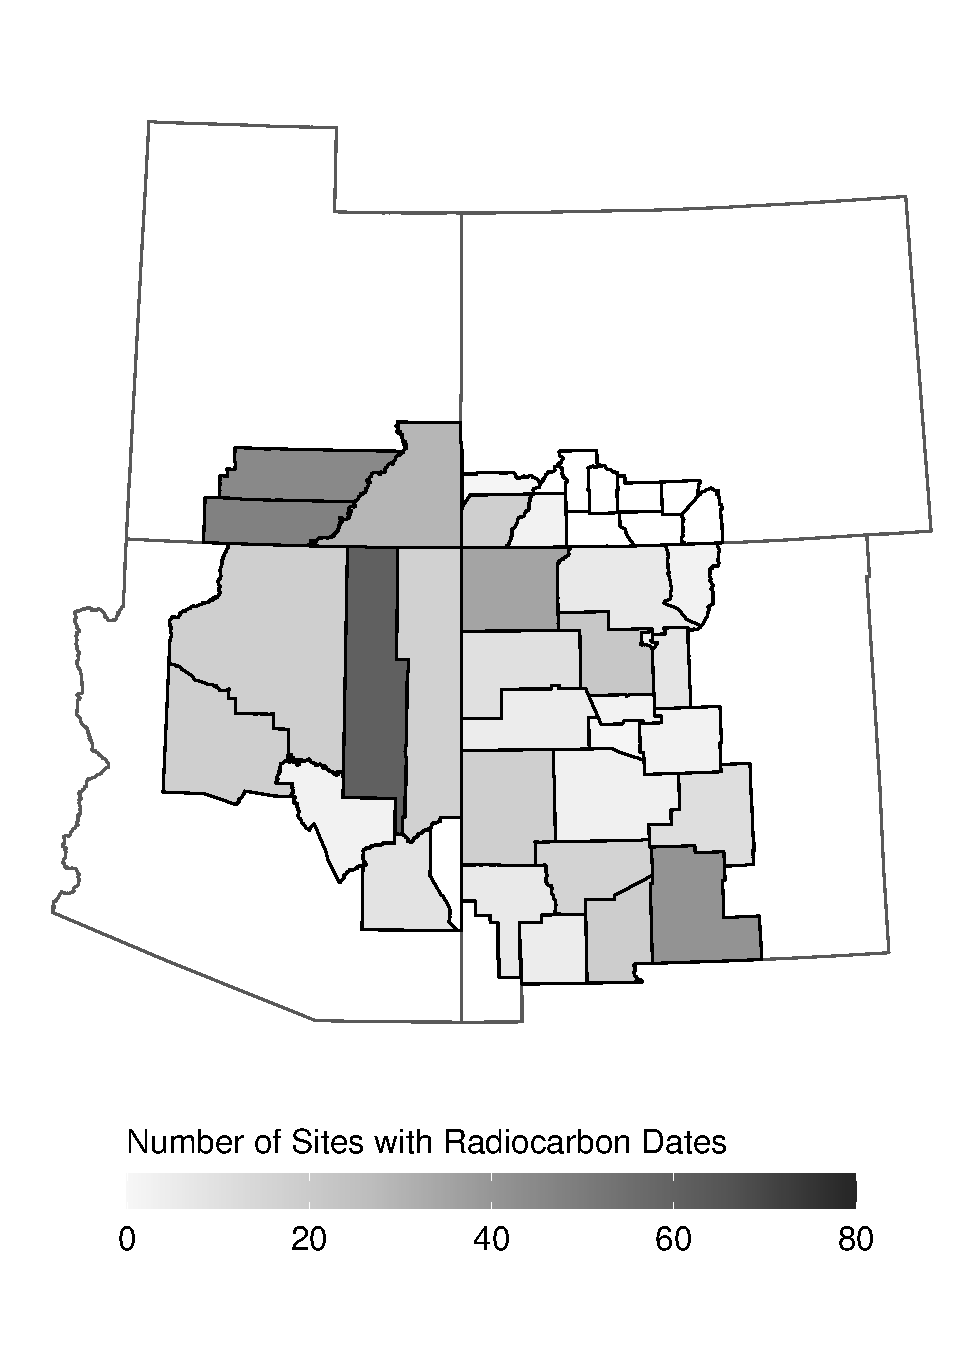
\includegraphics[width=0.45\linewidth]{/Users/bocinsky/git/publications/robinson2020/analysis/figures/Figure3-1} 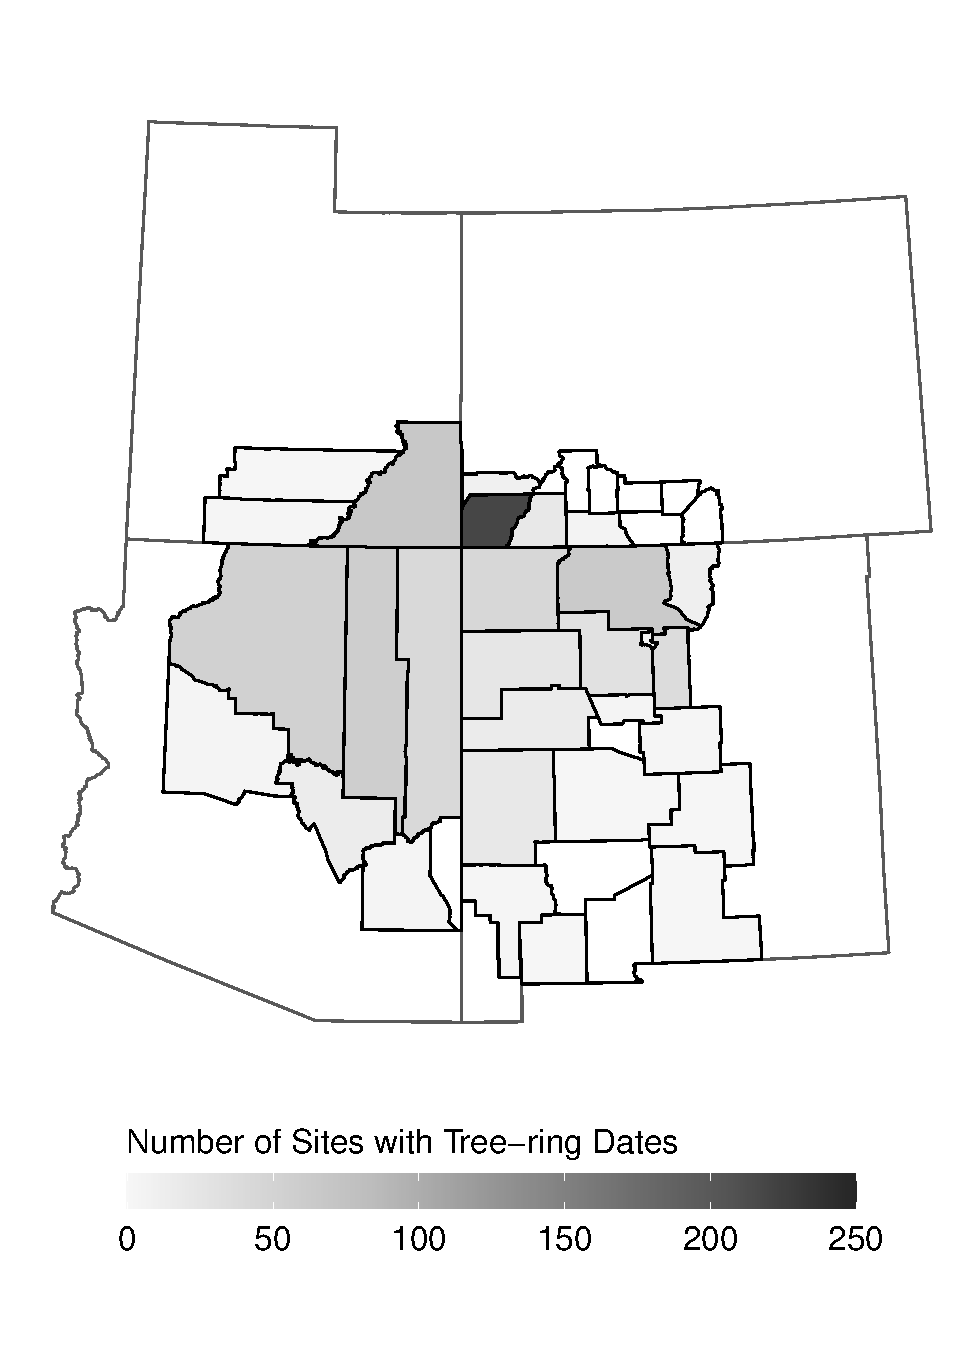
\includegraphics[width=0.45\linewidth]{/Users/bocinsky/git/publications/robinson2020/analysis/figures/Figure3-2} 

}

\caption{The number of sites with radiocarbon and tree-ring dates by county in this study.}\label{fig:Figure3}
\end{figure}

\hypertarget{preparing-the-spds}{%
\subsection*{Preparing the SPDs}\label{preparing-the-spds}}
\addcontentsline{toc}{subsection}{Preparing the SPDs}

To prepare the radiocarbon dataset, we used functions provided by the rcarbon package for R (Bevan et al., \protect\hyperlink{ref-Bevan2019}{2019}). We calibrated the radiocarbon dates using the methods of Bronk Ramsey (\protect\hyperlink{ref-Bronk2008}{2008}), using the `intcal13' calibration curve (Reimer et al., \protect\hyperlink{ref-Reimer2013}{2013}). To control for the inconsistent number of dates among the archaeological sites represented in the database (a form of investigation bias), we aggregated radiocarbon dates known to be from the same phase of an archaeological site using the rcarbon::binPrep function using the single linkage agglomeration method with an h-value of 100 (see {[}Supplementary Material{]} for a discussion of various h-values). This creates clusters of dates from the same site whose mean values (uncalibrated) are within 100 years of each other, and splits site occupations into distinct phases separated by 100 years or more. We constructed summed probability distributions (SPDs) from the calibrated dates using the \texttt{rcarbon::spd} function. We averaged probability distributions of binned dates, and then constructed SPDs from the resulting site-phase probability distributions.\footnote{Using this method, a site-phase with a single date and a site-phase with 10 dates would each contribute equally to the resulting SPD. This method of developing the SPD is therefore a model of the relative abundance of site occupation events through time rather than of dates through time. This method does not account for investigation biases deriving from the definition of ``site'' or the decision to use a particular dating technique at a site in the first place.}

We treated the tree-ring dates in as similar a way possible as the radiocarbon dates. We modeled faux-calibrated tree-ring date probabilities as discrete degenerate distributions (\(\Pr(X=k_0)=1\)) with \(k_0\) equal to the tree-ring date --- in other words, a probability of \(1\) at the date value, and \(0\) elsewhere. This is akin to modeling the tree ring date as a normal distribution with a mean of the date value, and a standard deviation of zero. Thinking of tree ring dates this way allows us to use the same binning and SPD algorithms as for radiocarbon dates.\footnote{One might consider alternative probability distributions for non-cutting or near-cutting dates. The probability mass function in such a case would be zero for years prior to the date of the outer ring of the sample, and non-zero for subsequent years, presumably decaying quickly. For instance, we could imagine a study that derives empirical probability distributions for non-cutting dates based on cutting-dates from the same contexts.} Here, we binned the tree-ring dates into site-phases using the rcarbon::binPrep function and constructing SPDs using \texttt{rcarbon::spd}, both with the same parameter selections as used for the radiocarbon samples. As above, we averaged probability distributions of binned dates, and then constructed SPDs from the site-phase distributions.

\hypertarget{results}{%
\section*{Results}\label{results}}
\addcontentsline{toc}{section}{Results}

Figure \ref{fig:Figure4} presents radiocarbon and tree-ring SPDs for the UUSW, CMV, and NRG regions, as well as VEP population reconstructions for the CMV and NRG regions. Across the UUSW, we see striking agreement in directionality and timing between the radiocarbon and tree-ring series (Figure \ref{fig:Figure4}A); both series trend upwards until the late thirteenth century, and then decline rapidly. The tree-ring series --- the light orange line is the raw SPD, and the dark line is smoothed --- shows more variation on annual to decadal timescales, and yet matches the broad trends of the radiocarbon SPD. Roughly 150-year periodic fluctuations in the tree-ring SPD, described as periods of ``exploration'' and ``exploitation'' by Bocinsky et al. (\protect\hyperlink{ref-Bocinsky2016}{2016}), are not present in the radiocarbon SPD, the result of a much smaller sample size of site-phases and lower temporal resolution of radiocarbon dating relative to tree-ring dating.



\begin{figure}

{\centering 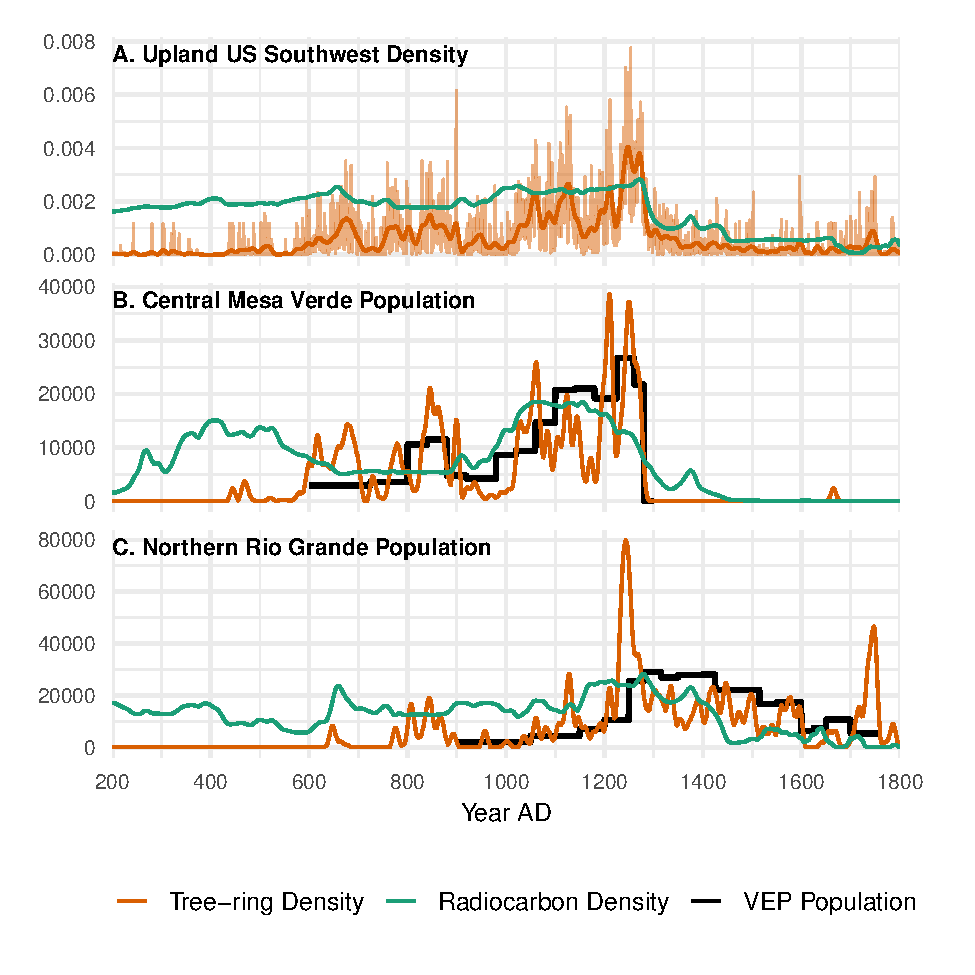
\includegraphics[width=0.75\linewidth]{/Users/bocinsky/git/publications/robinson2020/analysis/figures/Figure4-1} 

}

\caption{Radiocarbon and tree-ring density distributions in the UUSW (A), CMV (B), and NRG (C) regions, and VEP population estimates for the CMV and NRG. The dark orange tree-ring density curve smooths the raw tree-ring density (light orange) using a 21-year center-aligned Gaussian kernel with a 5-year standard deviation, following Bocinsky et al. (\protect\hyperlink{ref-Bocinsky2016}{2016}). In Panel A, the radiocarbon density (y-axis) is scaled by a factor of 3 to facilitate comparison with the tree-ring density over the target time period. The radiocarbon and tree-ring densities (y-axis) in panels B and C are scaled such that the area under their densities is equal to the area under the VEP population estimates (i.e., the cumulative population).}\label{fig:Figure4}
\end{figure}

Comparisons between the CMV and NRG regional SPDs and the VEP population estimates are also revealing. In Figures \ref{fig:Figure4}B and \ref{fig:Figure4}C, the regional SPDs have been scaled such that the areas under their densities (the orange and green lines) are equal to the area under the VEP population estimates (the black lines). For both regions, the radiocarbon and tree-ring SPDs capture the broad directionality of the VEP population estimates. In the CMV region (Figure \ref{fig:Figure4}B), the radiocarbon SPD has substantial probability mass prior to the VEP reconstruction, which is likely due to sampling bias in the radiocarbon record that is skewed in this region towards older (pre-Pueblo) sites. The radiocarbon SPD also does not capture the Pueblo I (AD 750--900) population peak (which may be too short-lived to be captured by such a small sample of radiocarbon dates), and seems to begin declining by the early thirteenth century AD. The tree-ring SPDs better capture the variability in population, though include a decline in the mid AD 1100s that is not in the VEP population estimates. In the NRG region (Figure \ref{fig:Figure4}C), both SPDs rise until about AD 1250, then decline thereafter. The high peak in the tree-ring record at AD 1250, far in excess of the VEP population estimate, is particularly interesting --- it likely signals the net impact of the immigration of many thousands of people to the NRG region, and the resulting (and simultaneous) burst in construction. Such a sudden and synchronous demographic and architectural event is hard to capture in the relatively lower resolution and sparsely sampled radiocarbon record, which tends to be smeared across sub-centennial scales courtesy of the calibration process (Baillie, \protect\hyperlink{ref-Baillie1991}{1991}).

These results yield key insights on the relative sensitivity of the radiocarbon record to capture long-term, coarse-grained demographic change across the Southwest. As stated in the introduction, our aim is to understand how well the radiocarbon record captures population declines across the Southwest, as we need to develop a measure of confidence in radiocarbon records from regions across and beyond the Southwest that lack other demographic proxies. Both the radiocarbon and tree-ring SPDs show declines post-AD 1300 across all regions. In both the CMV and NRG the decline in the radiocarbon SPD begins earlier than in the VEP population series. This may indicate that radiocarbon time series make the decline seem to begin earlier than it actually does, which could be caused by a `cliff' in the radiocarbon calibration curve from AD 1200--1300 that is surrounded by two plateaus at AD 1100--1200 and AD 1400 (Reimer et al., \protect\hyperlink{ref-Reimer2013}{2013}).

Comparisons of the radiocarbon and dendrochronological record with the architecture/ceramic record show similarities and differences that reinforce the need for multiple-proxy studies of palaeodemography when moving between broader and finer spatial scales. While the multi-proxy population reconstruction for the CMV region was similar to the radiocarbon and dendrochronological records, it showed a different trend for the NRG region (lower panel, Figure \ref{fig:Figure4}). There, the population reconstruction peaks from AD 1300--1400, whereas the radiocarbon record declines, at first quickly and then slowly. These different trends between the VEP population reconstructions and dendrochronological and radiocarbon proxies reflect some investigation bias in both the radiocarbon and dendrochronological records at smaller, intra-regional scales, which calls for caution in the use of radiocarbon records to assess possible paleo-migration scenarios at finer spatial scales. This result reinforces other work that has called for the use of multiple proxies as cross-checks on radiocarbon time series (Williams, \protect\hyperlink{ref-Williams2012}{2012}, p. @Crombe2014).

The central aim in comparing radiocarbon to dendrochronological records here was to assess the potential impacts of investigation bias in radiocarbon records, caused by researchers not taking radiocarbon samples in favour of other types of chronometric techniques (e.g., diagnostic artefact counts, tree-ring dates). Specifically, we are interested in the potential impact of this kind of bias in the post AD 1300 decline of radiocarbon SPDs across and beyond the Southwest. Similarities in the decline of both radiocarbon and dendrochronological records across the UUSW suggest that, at this particular regional scale, radiocarbon records reflect long-term, coarse-grained trends in paleodemography. Indeed, not only do we see corresponding declines in the radiocarbon and dendrochronological records at this large scale, but these patterns are also consistent with previous work on demographic and social change in the American Southwest: the Coalescent Communities Database, a Southwest-wide database of room counts and occupation spans of habitation sites with 12 rooms or more, supports a ``population decline that began between AD 1300 and 1350 and continued to European contact'' (Phillips et al., \protect\hyperlink{ref-Phillips2018}{2018}; following Hill et al., \protect\hyperlink{ref-Hill2004}{2004}: Figures 2,4).

\hypertarget{conclusion}{%
\section*{Conclusion}\label{conclusion}}
\addcontentsline{toc}{section}{Conclusion}

Understanding the geographic scale of post-AD 1300 human population declines in the American Southwest requires a reliance on radiocarbon-based reconstructions of palaeodemography, as radiocarbon is often the only proxy record available in many regions for developing continuous time series. However, radiocarbon records may include investigation bias caused by researchers not selecting radiocarbon samples in favour of Late Prehistoric diagnostic artefacts or other dating methods. In this paper we develop a new method for systematically comparing radiocarbon time series against multiple palaeodemographic proxies. We selected three regions---the Upland US Southwest, Central Mesa Verde, and the Northern Rio Grande---where we expected the most investigation bias to occur, because in these regions multiple higher resolution dating techniques are available. Results indicated that all three palaeodemographic proxies reveal post-AD 1300 population declines. While there is some variability at finer spatial and temporal scales that warrant the collection of other data that can be used to cross-check and validate the resolution of radiocarbon records, at coarse-grained, large spatial and temporal scales radiocarbon records provide a robust relative measure of long-term palaeodemographic trends. These results lend confidence to single proxy radiocarbon-based reconstructions of palaeodemography outside the Southwest that suggest post-AD 1300 population declines in many parts of North America.

Investigation bias is an inevitable issue that all researchers using radiocarbon records have to address. The results of this paper advance our confidence in radiocarbon records as a coarse-grained measure of the directionality of human paleodemographic trends. The methods developed can be used for other regions of the world that have dendrochronological records, such as Europe (Haneca et al., \protect\hyperlink{ref-Haneca2009}{2009}; Hillam et al., \protect\hyperlink{ref-Hillam1990}{1990}; Kuniholm, \protect\hyperlink{ref-Kuniholm2001}{2001}), where comparisons with radiocarbon records could help to advance knowledge of Neolithic `booms and busts' of populations (Shennan et al., \protect\hyperlink{ref-Shennan2013}{2013}; Whitehouse et al., \protect\hyperlink{ref-Whitehouse2014}{2014}) and to overcome limitations of the Bronze Age radiocarbon calibration plateau (Armit et al., \protect\hyperlink{ref-Armit2013}{2013}).

\hypertarget{acknowledgements}{%
\paragraph*{Acknowledgements}\label{acknowledgements}}
\addcontentsline{toc}{paragraph}{Acknowledgements}

We thank the guest editorial board for inviting us to contribute to this volume. We thank two anonymous reviewers for their helpful suggestions for improvement. We thank our colleagues in the PAGES People3000 working group, and PAGES for funding this working group. We thank the National Foundation for supporting this research. Lastly, we thank the generations of different stakeholders working across the Southwest for their collection, storage and publication of the data presented here.

\hypertarget{data-accessibility}{%
\paragraph*{Data Accessibility}\label{data-accessibility}}
\addcontentsline{toc}{paragraph}{Data Accessibility}

A compendium of data and code used in this analysis is available on Github at \url{https://github.com/people3k/robinson2020} and is archived with Zenodo at \url{https://doi.org/10.5281/zenodo.3647599}. Radiocarbon data used in this analysis are archived with the Digital Archaeological Record (tDAR) and are available at \url{https://doi.org/10.6067/XCV8455460}. Tree-ring data used here are archived with tDAR at \url{https://doi.org/10.6067/XCV82J6D7B}. Archaeological site locations are protected by US federal and state statutes. In order to protect these sensitive data, we pre-processed both the radiocarbon and tree-ring data; data included in the Github repository do not include site locations, and researchers will need to gain permission from the State Historic Preservation Office (SHPO) of each state in order to access the site location data.

\hypertarget{ethics}{%
\paragraph*{Ethics}\label{ethics}}
\addcontentsline{toc}{paragraph}{Ethics}

No ethical issues are associated with this paper.

\hypertarget{authors-contributions}{%
\paragraph*{Authors' contributions}\label{authors-contributions}}
\addcontentsline{toc}{paragraph}{Authors' contributions}

E.R. and R.K.B designed the study, collected and analysed the data, and wrote the first draft. J.F. and D.B collected and organized data. R.L.K collected data. All authors revised/improved the manuscript.

\hypertarget{competing-interests}{%
\paragraph*{Competing interests}\label{competing-interests}}
\addcontentsline{toc}{paragraph}{Competing interests}

We have no competing interests.

\hypertarget{funding}{%
\paragraph*{Funding}\label{funding}}
\addcontentsline{toc}{paragraph}{Funding}

Funding for this research was provided by NSF grants BCS-1418858, BCS-1624061, BCS-1822033 and PAGES (Past Global Changes) funding to the Working Group \href{http://www.pastglobalchanges.org/ini/wg/arctic2k/170-initiatives/working-group/people-3000/1732-people-3000}{Paleoclimate and the Peopling of the Earth (PEOPLE 3000)}.

\newpage

\hypertarget{references}{%
\section*{References}\label{references}}
\addcontentsline{toc}{section}{References}

\hypertarget{refs}{}
\begin{cslreferences}
\leavevmode\hypertarget{ref-Armit2013}{}%
Armit, I., Swindles, G.T., Becker, K., 2013. From dates to demography in later prehistoric Ireland? Experimental approaches to the meta-analysis of large \textsuperscript{14}C data-sets. Journal of archaeological science 40, 433--438. \url{https://doi.org/10.1016/j.jas.2012.08.039}

\leavevmode\hypertarget{ref-Baillie1991}{}%
Baillie, M.G., 1991. Suck-in and smear: Two related chronological problems for the 90s. Journal of theoretical archaeology 2, 12--16.

\leavevmode\hypertarget{ref-Bamforth2012}{}%
Bamforth, D.B., Grund, B., 2012. Radiocarbon calibration curves, summed probability distributions, and early Paleoindian population trends in North America. Journal of Archaeological Science 39, 1768--1774. \url{https://doi.org/10.1016/j.jas.2012.01.017}

\leavevmode\hypertarget{ref-Berry1982}{}%
Berry, M.S., 1982. Time, space and transition in anasazi prehistory. University of Utah Press, Salt Lake City, Utah.

\leavevmode\hypertarget{ref-rcarbon}{}%
Bevan, A., Crema, E.R., 2020. rcarbon: Methods for calibrating and analysing radiocarbon dates.

\leavevmode\hypertarget{ref-Bevan2019}{}%
Bevan, A., Palmisano, A., Woodbridge, J., Fyfe, R., Roberts, C.N., Shennan, S., 2019. The changing face of the Mediterranean---Land cover, demography and environmental change: Introduction and overview. The Holocene 29, 703--707. \url{https://doi.org/10.1177/0959683619826688}

\leavevmode\hypertarget{ref-Bluhm2019}{}%
Bluhm, L.E., Surovell, T.A., 2019. Validation of a global model of taphonomic bias using geologic radiocarbon ages. Quaternary Research 91, 325--328. \url{https://doi.org/10.1017/qua.2018.78}

\leavevmode\hypertarget{ref-Bocinsky2016}{}%
Bocinsky, R.K., Rush, J., Kintigh, K.W., Kohler, T.A., 2016. Exploration and exploitation in the macrohistory of the pre-Hispanic Pueblo Southwest. Science Advances 2, e1501532. \url{https://doi.org/10.1126/sciadv.1501532}

\leavevmode\hypertarget{ref-Boyer2010}{}%
Boyer, J.L., Moore, J.L., Lakatos, S.A., Akins, N.J., Wilson, C.D., Blinman, E., 2010. Remodeling immigration: A Northern Rio Grande perspective on depopulation, migration, and donation-side models, in: Kohler, T., Varien, M., Wright, A. (Eds.), Leaving Mesa Verde: Peril and Change in the Thirteenth Century Southwest. The Amerind Foundation; University of Arizona Press, Tucson, Arizona, pp. 285--323.

\leavevmode\hypertarget{ref-Bronk2008}{}%
Bronk Ramsey, C., 2008. Radiocarbon dating: Revolutions in understanding. Archaeometry 50, 249--275. \url{https://doi.org/10.1111/j.1475-4754.2008.00394.x}

\leavevmode\hypertarget{ref-Cameron2010}{}%
Cameron, C.M., 2010. Advances in understanding the thirteenth-century depopulation of the northern Southwest, in: Kohler, T., Varien, M., Wright, A. (Eds.), Leaving Mesa Verde: Peril and Change in the Thirteenth Century Southwest. The Amerind Foundation; University of Arizona Press, Tucson, Arizona, pp. 346--363.

\leavevmode\hypertarget{ref-Contreras2014}{}%
Contreras, D.A., Meadows, J., 2014. Summed radiocarbon calibrations as a population proxy: A critical evaluation using a realistic simulation approach. Journal of Archaeological Science 52, 591--608. \url{https://doi.org/10.1016/j.jas.2014.05.030}

\leavevmode\hypertarget{ref-Crema2016}{}%
Crema, E.R., Habu, J., Kobayashi, K., Madella, M., 2016. Summed probability distribution of \textsuperscript{14}C dates suggests regional divergences in the population dynamics of the Jomon period in eastern Japan. PLoS One 11, e0154809. \url{https://doi.org/10.1371/journal.pone.0154809}

\leavevmode\hypertarget{ref-Crombe2014}{}%
Crombé, P., Robinson, E., 2014. \textsuperscript{14}C dates as demographic proxies in Neolithisation models of northwestern Europe: A critical assessment using Belgium and northeast France as a case-study. Journal of Archaeological Science 52, 558--566. \url{https://doi.org/10.1016/j.jas.2014.02.001}

\leavevmode\hypertarget{ref-Freeman2018PNAS}{}%
Freeman, J., Baggio, J.A., Robinson, E., Byers, D.A., Gayo, E., Finley, J.B., Meyer, J.A., Kelly, R.L., Anderies, J.M., 2018. Synchronization of energy consumption by human societies throughout the Holocene. Proceedings of the National Academy of Sciences 115, 9962--9967. \url{https://doi.org/10.1073/pnas.1802859115}

\leavevmode\hypertarget{ref-Freeman2018}{}%
Freeman, J., Byers, D.A., Robinson, E., Kelly, R.L., 2018. Culture process and the interpretation of radiocarbon data. Radiocarbon 60, 453--467. \url{https://doi.org/10.1017/RDC.2017.124}

\leavevmode\hypertarget{ref-Goldberg2016}{}%
Goldberg, A., Mychajliw, A.M., Hadly, E.A., 2016. Post-invasion demography of prehistoric humans in South America. Nature 532, 232--235. \url{https://doi.org/10.1038/nature17176}

\leavevmode\hypertarget{ref-Haneca2009}{}%
Haneca, K., Čufar, K., Beeckman, H., 2009. Oaks, tree-rings and wooden cultural heritage: A review of the main characteristics and applications of oak dendrochronology in Europe. Journal of Archaeological Science 36, 1--11. \url{https://doi.org/10.1016/j.jas.2008.07.005}

\leavevmode\hypertarget{ref-Hill2004}{}%
Hill, J.B., Clark, J.J., Doelle, W.H., Lyons, P.D., 2004. Prehistoric demography in the Southwest: Migration, coalescence, and Hohokam population decline. American Antiquity 69, 689--716. \url{https://doi.org/10.2307/4128444}

\leavevmode\hypertarget{ref-Hillam1990}{}%
Hillam, J., Groves, C.M., Brown, D.M., Baillie, M.G., Coles, J.M., Coles, B.J., 1990. Dendrochronology of the English Neolithic. Antiquity 64, 210--220. \url{https://doi.org/10.1017/S0003598X00077826}

\leavevmode\hypertarget{ref-Kohler2010b}{}%
Kohler, T.A., Varien, M.D., Wright, A.M. (Eds.), 2010. Leaving Mesa Verde: Peril and Change in the Thirteenth-Century Southwest. The Amerind Foundation; University of Arizona Press, Tucson, Arizona.

\leavevmode\hypertarget{ref-Kuniholm2001}{}%
Kuniholm, P.I., 2001. Dendrochronology and other applications of tree-ring studies in archaeology, in: Brothwell, D.R., Pollard, A.M. (Eds.), The Handbook of Archaeological Sciences. John Wiley \& Sons, Ltd., London.

\leavevmode\hypertarget{ref-rrtools}{}%
Marwick, B., 2019. rrtools: Creates a Reproducible Research Compendium.

\leavevmode\hypertarget{ref-Marwick2017}{}%
Marwick, B., 2017. Computational reproducibility in archaeological research: Basic principles and a case study of their implementation. Journal of Archaeological Method and Theory 24, 424--450. \url{https://doi.org/10.1007/s10816-015-9272-9}

\leavevmode\hypertarget{ref-Michczynski2006}{}%
Michczynski, A., Michczynska, D.J., 2006. The effect of PDF peaks' height increase during calibration of radiocarbon date sets. Geochronometria 25, 1--4.

\leavevmode\hypertarget{ref-Naudinot2014}{}%
Naudinot, N., Tomasso, A., Tozzi, C., Peresani, M., 2014. Changes in mobility patterns as a factor of \textsuperscript{14}C date density variation in the Late Epigravettian of Northern Italy and Southeastern France. Journal of Archaeological Science 52, 578--590. \url{https://doi.org/10.1016/j.jas.2014.05.021}

\leavevmode\hypertarget{ref-Ortman2016}{}%
Ortman, S.G., 2016. Uniform probability density analysis and population history in the northern Rio Grande. Journal of Archaeological Method and Theory 23, 95--126. \url{https://doi.org/10.1007/s10816-014-9227-6}

\leavevmode\hypertarget{ref-Palmisano2019}{}%
Palmisano, A., Woodbridge, J., Roberts, C.N., Bevan, A., Fyfe, R., Shennan, S., Cheddadi, R., Greenberg, R., Kaniewski, D., Langgut, D., others, 2019. Holocene landscape dynamics and long-term population trends in the Levant. The Holocene 29, 708--727. \url{https://doi.org/10.1177/0959683619826642}

\leavevmode\hypertarget{ref-Peros2010}{}%
Peros, M.C., Munoz, S.E., Gajewski, K., Viau, A.E., 2010. Prehistoric demography of North America inferred from radiocarbon data. Journal of Archaeological Science 37, 656--664. \url{https://doi.org/10.1016/j.jas.2009.10.029}

\leavevmode\hypertarget{ref-Phillips2018}{}%
Phillips, D.A., Wearing, H.J., Clark, J.J., 2018. Village growth, emerging infectious disease, and the end of the Neolithic Demographic Transition in the Southwest United States and Northwest Mexico. American Antiquity 83, 263--280. \url{https://doi.org/10.1017/aaq.2018.3}

\leavevmode\hypertarget{ref-Reimer2013}{}%
Reimer, P.J., Bard, E., Bayliss, A., Beck, J.W., Blackwell, P.G., Ramsey, C.B., Buck, C.E., Cheng, H., Edwards, R.L., Friedrich, M., others, 2013. IntCal13 and Marine13 radiocarbon age calibration curves 0--50,000 years cal BP. Radiocarbon 55, 1869--1887. \url{https://doi.org/10.2458/azu_js_rc.55.16947}

\leavevmode\hypertarget{ref-Rick1987}{}%
Rick, J.W., 1987. Dates as data: An examination of the Peruvian preceramic radiocarbon record. American Antiquity 52, 55--73. \url{https://doi.org/10.2307/281060}

\leavevmode\hypertarget{ref-Robinson2019}{}%
Robinson, E., Nicholson, C., Kelly, R.L., 2019. The importance of spatial data to open-access national archaeological databases and the development of paleodemography research. Advances in Archaeological Practice 7, 395--408. \url{https://doi.org/10.1017/aap.2019.29}

\leavevmode\hypertarget{ref-Russell2009}{}%
Russell, T., Steele, J., 2009. A geo-referenced radiocarbon database for Early Iron Age sites in sub-Saharan Africa: Initial analysis. Southern African Humanities 21, 327--344.

\leavevmode\hypertarget{ref-Schwindt2016}{}%
Schwindt, D.M., Bocinsky, R.K., Ortman, S.G., Glowacki, D.M., Varien, M.D., Kohler, T.A., 2016. The social consequences of climate change in the central Mesa Verde region. American Antiquity 81, 74--96.

\leavevmode\hypertarget{ref-Shennan2013}{}%
Shennan, S., Downey, S.S., Timpson, A., Edinborough, K., Colledge, S., Kerig, T., Manning, K., Thomas, M.G., 2013. Regional population collapse followed initial agriculture booms in mid-holocene europe. Nature communications 4, 1--8.

\leavevmode\hypertarget{ref-Surovell2007}{}%
Surovell, T.A., Brantingham, P.J., 2007. A note on the use of temporal frequency distributions in studies of prehistoric demography. Journal of Archaeological Science 34, 1868--1877.

\leavevmode\hypertarget{ref-Surovell2009}{}%
Surovell, T.A., Finley, J.B., Smith, G.M., Brantingham, P.J., Kelly, R., 2009. Correcting temporal frequency distributions for taphonomic bias. Journal of archaeological Science 36, 1715--1724.

\leavevmode\hypertarget{ref-Timpson2014}{}%
Timpson, A., Colledge, S., Crema, E., Edinborough, K., Kerig, T., Manning, K., Thomas, M.G., Shennan, S., 2014. Reconstructing regional population fluctuations in the european neolithic using radiocarbon dates: A new case-study using an improved method. Journal of Archaeological Science 52, 549--557.

\leavevmode\hypertarget{ref-Wang2014}{}%
Wang, C., Lu, H., Zhang, J., Gu, Z., He, K., 2014. Prehistoric demographic fluctuations in china inferred from radiocarbon data and their linkage with climate change over the past 50,000 years. Quaternary Science Reviews 98, 45--59.

\leavevmode\hypertarget{ref-Whitehouse2014}{}%
Whitehouse, N.J., Schulting, R.J., McClatchie, M., Barratt, P., McLaughlin, T.R., Bogaard, A., Colledge, S., Marchant, R., Gaffrey, J., Bunting, M.J., 2014. Neolithic agriculture on the European western frontier: The boom and bust of early farming in Ireland. Journal of Archaeological Science 51, 181--205.

\leavevmode\hypertarget{ref-Williams2012}{}%
Williams, A.N., 2012. The use of summed radiocarbon probability distributions in archaeology: A review of methods. Journal of Archaeological Science 39, 578--589.
\end{cslreferences}

\newpage

\hypertarget{supplementary-material-cut-width-sensitivity-for-temporal-binning}{%
\section*{Supplementary Material: Cut-width sensitivity for temporal binning}\label{supplementary-material-cut-width-sensitivity-for-temporal-binning}}
\addcontentsline{toc}{section}{Supplementary Material: Cut-width sensitivity for temporal binning}

Uneven sampling across archaeological contexts is a persistant problem when constructing summed probability distributions from radiocarbon dates, and perhaps even a larger issue for the more ubiquitous tree-ring dates in regions like the Upland US Southwest. In SPDs of radiocarbon dates, it is conventional to combine dates from single sites prior to creating the SPDs. Dates from separate components or phases of multi-component sites should be counted separately, however.

To control for inconsistent sample size across the archaeological sites represented in the database, we aggregated dates known to be from the same phase of same archaeological site using the \texttt{rcarbon::binPrep} function using the ``single linkage'' agglomeration method with a cut width (or \(h\)-value) of 100 (Bevan and Crema, \protect\hyperlink{ref-rcarbon}{2020}). This clusters dates from the same site that are within 100 years of each other, and splits site occupations into distinct phases separated by 100 years or more. Binned calibrated dates are then summed, and the resulting probability mass function is divided by the number of dates in the site-phase.

Because the wider archaeological SPD research community still lacks a standard protocol for determining \(h\), we perform a sensitivity analysis to demonstrate that the resulting SPDs for radiocarbon and tree-ring dates stabilize at a cut width of 100 or so. We calculated SPDs at 25-year intervals from 0 (only duplicate dates are binned) to 150 years (effectively binning by site).

As can be seen in Figure \ref{fig:FigureS1}, binning in general has little impact on the resulting SPDs, but cut widths above \(h=100\) years are virtually indistinguishable. The shape of the radiocarbon SPD (panel A) stabilizes above \(h=0\) and its values stabilize by \(h=100\). The tree-ring SPD arguably stabilizes in both shape and value above \(h=75\) or so, but in the analysis we use \(h=100\) to keep our methods consistent between the radiocarbon and tree-ring SPDs.

\begin{figure}

{\centering 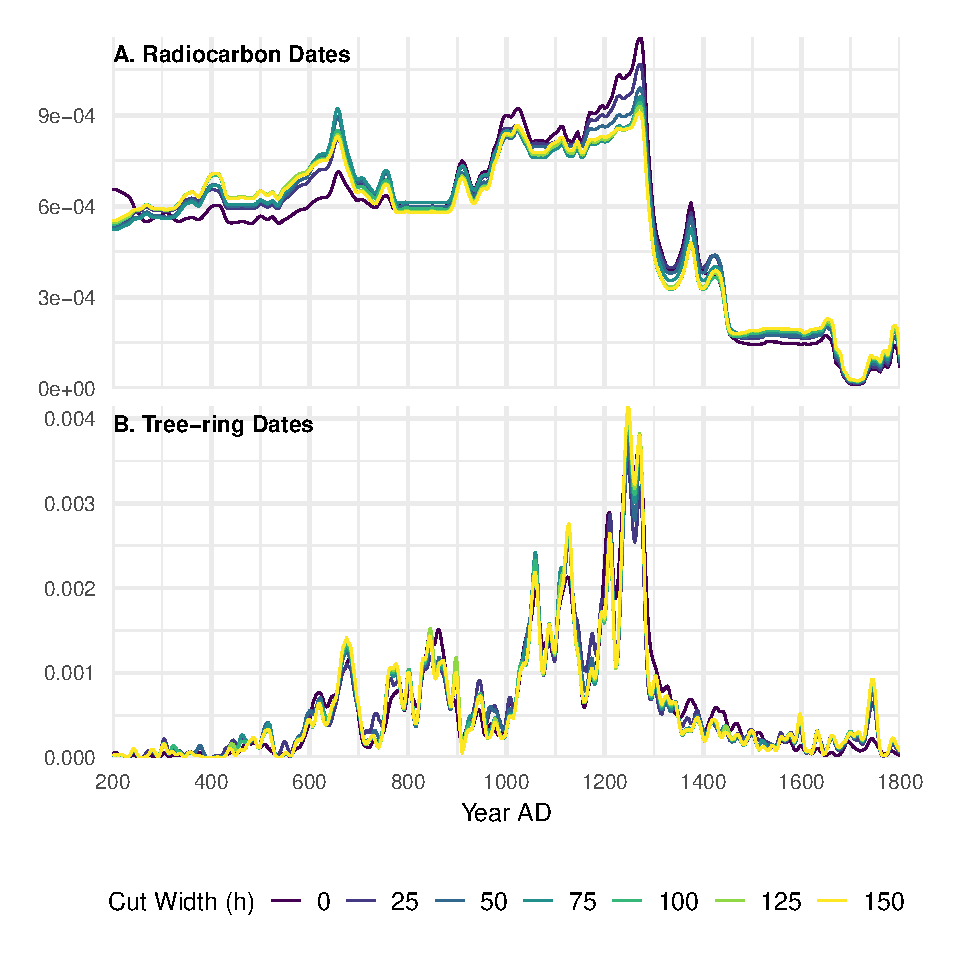
\includegraphics[width=0.75\linewidth]{/Users/bocinsky/git/publications/robinson2020/analysis/figures/FigureS1-1} 

}

\caption{Radiocarbon (A) and tree-ring (B) density distributions in the UUSW, given varying cut widths for binning dates within sites. The density distributions for the UUSW are normalized. Years are given in AD.}\label{fig:FigureS1}
\end{figure}

\newpage

\hypertarget{colophon}{%
\section*{Colophon}\label{colophon}}
\addcontentsline{toc}{section}{Colophon}

This report is part of a research compendium developed using the \texttt{rrtools} package for reproducible research (Marwick, \protect\hyperlink{ref-rrtools}{2019}, \protect\hyperlink{ref-Marwick2017}{2017}). This report was generated on 2020-04-17 11:04:15 using the following computational environment and dependencies:

\textbf{R version 3.6.3 (2020-02-29)}

\textbf{Platform:} x86\_64-apple-darwin15.6.0 (64-bit)

\textbf{locale:}
en\_US.UTF-8\textbar\textbar en\_US.UTF-8\textbar\textbar en\_US.UTF-8\textbar\textbar C\textbar\textbar en\_US.UTF-8\textbar\textbar en\_US.UTF-8

\textbf{attached base packages:}
\emph{stats}, \emph{graphics}, \emph{grDevices}, \emph{utils}, \emph{datasets}, \emph{methods} and \emph{base}

\textbf{other attached packages:}
\emph{ggplot2(v.3.3.0)}, \emph{robinson2020(v.1.0.0.9000)} and \emph{magrittr(v.1.5)}

\textbf{loaded via a namespace (and not attached):}
\emph{Rcpp(v.1.0.4)}, \emph{compiler(v.3.6.3)}, \emph{pillar(v.1.4.3)}, \emph{tools(v.3.6.3)}, \emph{digest(v.0.6.25)}, \emph{evaluate(v.0.14)}, \emph{lifecycle(v.0.2.0)}, \emph{tibble(v.3.0.0)}, \emph{gtable(v.0.3.0)}, \emph{pkgconfig(v.2.0.3)}, \emph{rlang(v.0.4.5)}, \emph{cli(v.2.0.2)}, \emph{yaml(v.2.2.1)}, \emph{xfun(v.0.13)}, \emph{withr(v.2.1.2)}, \emph{stringr(v.1.4.0)}, \emph{dplyr(v.0.8.5)}, \emph{knitr(v.1.28)}, \emph{vctrs(v.0.2.4)}, \emph{rprojroot(v.1.3-2)}, \emph{grid(v.3.6.3)}, \emph{tidyselect(v.1.0.0)}, \emph{glue(v.1.4.0)}, \emph{here(v.0.1)}, \emph{R6(v.2.4.1)}, \emph{fansi(v.0.4.1)}, \emph{rmarkdown(v.2.1)}, \emph{bookdown(v.0.18)}, \emph{pander(v.0.6.3)}, \emph{purrr(v.0.3.3)}, \emph{backports(v.1.1.6)}, \emph{scales(v.1.1.0)}, \emph{ellipsis(v.0.3.0)}, \emph{htmltools(v.0.4.0)}, \emph{assertthat(v.0.2.1)}, \emph{colorspace(v.1.4-1)}, \emph{stringi(v.1.4.6)}, \emph{munsell(v.0.5.0)} and \emph{crayon(v.1.3.4)}

\end{document}
